\documentclass[12pt, reqno, a4paper]{amsart}
\usepackage{latexsym,fancyheadings,amsmath,amssymb,amsthm,amsbsy,graphicx, cite, floatrow,subcaption}
\usepackage[symbol]{footmisc}
\usepackage{hyperref}
\usepackage{mathrsfs}
\usepackage[utf8]{inputenc}
\usepackage[T2A]{fontenc}
\usepackage[english,ukrainian]{babel}

\usepackage{floatrow}
\floatsetup[table]{capposition=top}
\floatsetup[figure]{capposition=bottom,%
capbesideposition={right,bottom},%
capbesidewidth=0.3\textwidth,%
capbesidesep=quad% розділювач між картинкою та підписом
}

\textwidth = 13.1cm
\textheight = 21cm
\topmargin = 0cm
\headheight = 1cm

\theoremstyle{definition}
\newtheorem{defin}{Означення}
\theoremstyle{plain}
\newtheorem{theorem}{Теорема}
\theoremstyle{plain}
\newtheorem{lemma}{Лема}
\theoremstyle{plain}
\newtheorem{corollary}{Наслідок}
\theoremstyle{remark}
\newtheorem*{remark}{Зауваження}
\theoremstyle{plain}
\newtheorem{state}{Твердження}


\newcommand{\argmin}{\mathop{\rm argmin}\nolimits}
\newcommand{\prox}{\mathop{\rm prox}\nolimits}
\newcommand{\diver}{\mathop{\rm div}\nolimits}
\newcommand{\dom}{\mathop{\rm dom}\nolimits}
\newcommand{\diam}{\mbox{\rm diam}}
\newcommand{\conv}{\mbox{\rm conv}}
\newcommand{\supp}{\mbox{\rm supp}}
\newcommand{\inter}{\mbox{\rm int}}
\newcommand{\gr}{\mbox{\rm grad}}
\newcommand{\ri}{\mbox{\rm ri}}

\begin{document}

\newcommand{\FirstLeftHeader}[1]{\lhead{\fancyplain{\footnotesize #1}{}}}
\newcommand{\Headers}[2]{\chead[\fancyplain{}{\footnotesize #1}]{\fancyplain{}{\footnotesize #2}}}
\newcommand{\NoPageNumbers}{\cfoot{}}
\newcommand{\FirstRightHeader}[1]{\rhead{\fancyplain{\footnotesize #1} {}}}
\newcommand{\AuthorInfo}[1]{\bigskip \noindent {\sc #1}\bigskip}
\newcommand{\Caption}[2]{\medskip\begin{center}{\sc #1} #2\end{center}\smallskip}

\makeatletter
\renewcommand{\labelenumi}{\theenumi.}
\renewcommand{\labelitemi}{ -- }
\renewcommand{\@biblabel}[1]{#1.\hfill}
\renewcommand{\refname}{\sc Література}



\newenvironment{Abstract} { \vspace{-2pt}
 \begin{quote}\footnotesize \selectlanguage{english}{\sc Abstract.} }
 {\selectlanguage{ukrainian}\end{quote}\vspace{-4pt}}
\newenvironment{Abstract_u} {
 \begin{quote}\footnotesize \sloppy {\sc Анотація.} }
 {\end{quote}\vspace{-4pt}}
\newenvironment{Udc}{\begin{flushleft} УДК}
 {\end{flushleft}\vspace{-4pt}}
\newenvironment{MSC}{\begin{flushleft} MSC}
 {\end{flushleft}\vspace{-4pt}}
\newenvironment{Doi}{\begin{flushleft} DOI}
 {\end{flushleft}}
\newenvironment{Title}{\vspace{2pt} \bf \begin{center}}
 {\end{center}\vspace{-2pt}}
\newenvironment{Authors}{\vspace{2pt} \sc \begin{center}}
 {\end{center}\vspace{-2pt}}
\newenvironment{Head}{\vspace{10pt} \sc \begin{center}}
 {\end{center}}




\newcommand\blfootnote[1]{
    \begingroup
    \renewcommand\thefootnote{}\footnote{#1}
    \addtocounter{footnote}{-1}
    \endgroup
}


\pagestyle{fancyplain} \thispagestyle{plain}
\FirstLeftHeader{Журнал обчислювальної та\ \ \ \ \ \ \ \ \
\textbf{2026, № * (***)}\\прикладної математики}
\FirstRightHeader{Journal of Numerical \\ \& Applied
Mathematics}

\newcommand {\R} {\mathbb{R}}
\newcommand{\FrDer}[2][0]{\ensuremath{\mathcal{D}_{#1}^{#2}}}
\newcommand{\COmega}{C\left(\overline\Omega\right)}

%---------------------ПОЧАТОК СТАТТІ--------------------------

 {\small
%---------------------Парні та непарні колонтитули------------
  \Headers{В. В. ПЛАТОНОВ, Є. В. ПЛАТОНОВА}{МОДЕЛЮВАННЯ МУЛЬТИАГЕНТНОЇ ОРКЕСТРАЦІЇ}
  \NoPageNumbers

%---------------------УДК-------------------------------------
\begin{Udc}
 519.816, 004.896 \blfootnote{\copyright 2026 \textbf{Віталій Платонов}, \textbf{Євгенія Платонова}. This is an open-access article distributed under the terms of \textbf{Creative Commons Attribution Licence (CC BY)}.}
\end{Udc}
%---------------------MSC-------------------------------------
\begin{MSC}
 90C40, 60G40, 68T42, 68N30
\end{MSC}

%---------------------ЗАГОЛОВОК СТАТТІ АНГЛІЙСЬКОЮ------------
\begin{Title}
MODELLING OF THE ``FOUR ROOMS'' MULTI-AGENT ORCHESTRATION: SYSTEMS ANALYSIS APPROACH TO SOLVING COMPLEX DESIGN TASKS
\end{Title}
%---------------------АВТОРИ АНГЛІЙСЬКОЮ-----------------------
  \begin{Authors}
      {V. V. Platonov${\mathstrut}^1$\footnote[1]{corresponding author}, Ye. V. Platonova${\mathstrut}^1$}
  \end{Authors}

%---------------------Організації АНГЛІЙСЬКОЮ-----------------------
{\scriptsize \noindent ${\mathstrut}^1$Department of Optimal Control and Economic Cybernetics, Odesa I. I. Mechnikov National University, Odesa, Ukraine, E-mail: vitaly.platonov@gmail.com, jane.platonova@gmail.com. ORCID: 0000-0000-0000-0000.
\par}


%---------------------ЗАГОЛОВОК СТАТТІ УКРАЇНСЬКОЮ------------
 \begin{Title}
МОДЕЛЮВАННЯ МУЛЬТИАГЕНТНОЇ ОРКЕСТРАЦІЇ <<ЧОТИРИ КІМНАТИ>>: СИСТЕМНО-АНАЛІТИЧНИЙ ПІДХІД ДО ЗАВДАНЬ ПРОЕКТУВАННЯ
 \end{Title}

%---------------------АВТОРИ УКРАЇНСЬКОЮ-----------------------
  \begin{Authors}
{В. В. Платонов${\mathstrut}^1$, Є. В. Платонова${\mathstrut}^1$}
  \end{Authors}

%---------------------Організації УКРАЇНСЬКОЮ-----------------------
{\scriptsize \noindent ${\mathstrut}^1$Кафедра оптимального керування та економічної кібернетики, Одеський національний університет імені І. І. Мечникова, Одеса, Україна, E-mail: vitaly.platonov@gmail.com, jane.platonova@gmail.com. ORCID: 0000-0000-0000-0000.
}

%---------------------РЕЗЮМЕ АНГЛІЙСЬКОЮ-----------------------
\begin{Abstract}
\textit{The aim of the article} is to formalize the ``Four Rooms'' multi-agent orchestration framework for system design.
\textit{Research methodology.} The process is modelled as a finite-horizon Markov Decision Process (MDP) on an augmented state space with role isolation and verification via GraphSAGE, DiffPool, and Z3.
\textit{Results of the research.} A complexity metric $\Omega(T)$, an optimal stopping policy $\pi^*(s)$, and a decay bound $d \le (\delta / T_0)^{1/T_{\max}} \approx 0.89$ are derived. Across 50 projects, context compression reaches $R_{\text{c}} = 0.82$ while preserving $95.2\%$ of dependencies ($\sigma = 0.018$).
\textit{Practical significance.} Context burnout (\textit{token bleed}) is eliminated, ensuring design safety.
    \\
{\sc Keywords:} multi-agent orchestration, Markov decision process, optimal stopping, semantic compression.
\end{Abstract}

%---------------------РЕЗЮМЕ УКРАЇНСЬКОЮ-----------------------
\begin{Abstract_u}
\textit{Метою статті} є формалізація мультиагентного фреймворку <<Чотири кімнати>> для проектування інформаційних систем.
\textit{Методика дослідження.} Процес подано як марковський процес прийняття рішень (MDP) на розширеному просторі станів з ізоляцією ролей та верифікацією через GraphSAGE, DiffPool і Z3.
\textit{Результати дослідження.} Введено метрику $\Omega(T)$, обґрунтовано стратегію оптимальної зупинки $\pi^*(s)$ і межу згасання $d \le (\delta / T_0)^{1/T_{\max}} \approx 0.89$. На 50 проектах досягнуто стиснення контексту $R_{\text{c}} = 0.82$ при збереженні $95.2\%$ залежностей ($\sigma = 0.018$).
\textit{Практична значимість.} Усунено вигоряння контексту (\textit{token bleed}) і забезпечено цілісність специфікацій.
    \\
    {\sc Ключові слова:} мультиагентна оркестрація, марковський процес, оптимальна зупинка, семантичне стиснення.
  \end{Abstract_u}


{\scriptsize
\noindent
DOI: \href{doi.org/}{10.17721/2706-9699.}
\par}


%-------------------------ТЕКСТ СТАТТІ------------------------

\newpage


\begin{Head}
1. Вступ
\end{Head}

Широке впровадження автономних генеративних агентів у цикли розроблення програмного забезпечення оголило системні проблеми безпеки та схильності автогенераторів коду до внесення критичних дефектів, які були емпірично задокументовані у фундаментальних дослідженнях вразливостей систем генерації коду \cite{bib1}. У сучасних таксономіях безпеки автономних систем штучного інтелекту (ШІ) подібні аномалії класифікуються як специфічні режими відмов (\textit{failure modes}), спричинені накопиченням інформаційного шуму та розмиванням інструкцій у тривалих сесіях виконання \cite{bib2,bib3}. Показовим інженерним прецедентом став задокументований у липні 2025 року інцидент під час експерименту засновника SaaStr Джейсона Лемкіна з розроблення програмної системи за допомогою автономного ШІ-агента Replit \cite{bib4}. Попри явні текстові директиви заморозити будь-які зміни в конфігурації (\textit{Freeze}), агент внаслідок перевантаження та плутанини в лінійному контексті проігнорував обмеження і видалив робочу базу даних (\textit{production database}) із записами про понад 1200 компаній та 1200 менеджерів. Після виникнення помилки агент спробував замаскувати наслідки збою, згенерувавши понад 4000 фіктивних профілів користувачів та сфальсифікувавши звіти модульних тестів.

Цей прецедент демонструє ефект накопичення інформаційного шуму та ерозії жорстких обмежень через відсутність ізольованих фаз аналізу й детермінованих безпекових бар'єрів. Традиційні підходи до проектування систем за допомогою великих мовних моделей (LLM) намагаються компенсувати цю проблему лінійним розширенням вікна контексту. Проте зростання довжини вхідної послідовності посилює семантичну ентропію системи та підвищує ймовірність помилок генерації на стиках технологічних і бізнесових доменів. Для подолання цього бар'єра необхідний перехід від лінійного діалогового процесу до детермінованого скінченно-автоматного керування мультиагентним середовищем.

Такий перехід вимагає переосмислення класичного системного аналізу. Якщо у традиційній парадигмі суб'єктом проектування виступала людина, а об'єктом - інформаційна система, то в умовах автономного ШІ-проектування суб'єктом стає стохастичний обчислювальний агент, схильний до деградації уваги, дрейфу інструкцій (\textit{instruction drift}) та вигоряння контексту (\textit{token bleed}). Отже, математичний апарат оркестрації має моделювати фізичні та когнітивні обмеження самого обчислювального рушія (LLM) як структурну складову системної складності. Це формує теоретичну базу напряму \textbf{агентної системної інженерії (\textit{Agentic Systems Engineering})}, у якому аналітичні обмеження збіжності та формальні контури верифікації проектуються безпосередньо для контролю стохастичного ШІ-проектанта.

\begin{Head}
2. Огляд літератури
\end{Head}

Формалізація послідовного прийняття рішень в умовах стохастичної невизначеності спирається на класичний апарат навчання з підкріпленням Р. Саттона та Е. Барто \cite{bib5} і принцип оптимальності динамічного програмування Р. Беллмана \cite{bib6}. У роботах останніх років цей фундамент активно адаптується до моделювання автономних агентів на базі LLM: зокрема, досліджено теоретичні засади переходу від генерації токенів до простору дій у марковських середовищах \cite{bib7}, а також механізми балансування між дослідженням нових гіпотез та експлуатацією знайдених рішень (\textit{Exploration vs. Exploitation}) для мовних агентів \cite{bib8}.

Фізичні обмеження контекстного вікна трансформерних моделей детально вивчені у низці емпіричних робіт. Н. Лю зі співавторами довели наявність U-подібної кривої деградації уваги (\textit{Lost in the Middle}), через яку інформація в середині довгого контексту систематично втрачається моделлю \cite{bib9}. Для зменшення втрат під час складних міркувань М. Беста зі співавторами запропонували нелінійну парадигму графу думок (\textit{Graph of Thoughts, GoT}) \cite{bib10}, а стрес-тестування утримання ізольованих фактів (\textit{Needle In A Haystack}) підтвердило падіння точності відтворення інваріантів при заповненні контекстного вікна \cite{bib11}.

З метою структуризації простору проектування в інженерній практиці широко застосовується матриця дизайн-мислення Т. Брауна (IDEO) \cite{bib12}, яка розділяє вимоги за критеріями цінності, реалізованості та життєздатності. Водночас задача автоматизованого порівняння структурних специфікацій потребує методів векторного подання графів: індуктивного навчання вкладень вузлів GraphSAGE \cite{bib13}, диференційованого ієрархічного пулінгу DiffPool \cite{bib14} та метрик відстані між атрибутованими реляційними графами А. Санфеліу і К. Фу \cite{bib15}.

Серед сучасних архітектурних підходів до побудови багатоагентних систем виділяються декларативна компіляція мовних пайплайнів Stanford DSPy \cite{bib16}, евристичний пошук на деревах міркувань (\textit{Tree of Thoughts, ToT}) \cite{bib17} та асинхронна взаємодія агентів через спільну пам'ять за моделлю дошки оголошень (\textit{Blackboard Architecture}) Г. Нії \cite{bib18}. Для усунення стохастичних помилок генерації критично важливим є залучення детермінованих верифікаторів, таких як SMT-солвер Z3 Л. Де Моури та Н. Бйорнера \cite{bib19}, у поєднанні з формальними декларативними мовами опису інтерфейсів та інфраструктури - OpenAPI \cite{bib20}, OASIS TOSCA \cite{bib21} та HashiCorp HCL \cite{bib22}. Математичне обґрунтування правил зупинки ітераційних процесів базується на теорії дискретного стохастичного динамічного програмування М. Путермана \cite{bib23}, а семантичне узгодження текстових атрибутів вузлів забезпечується сіамськими трансформерними мережами Sentence-BERT \cite{bib24}.

Попри значний доробок у кожному з окремих напрямів, у наявній літературі залишається відкритою проблема синтезу цілісної моделі мультиагентної оркестрації, яка б одночасно забезпечувала марковську властивість процесу при мутаціях вимог, надавала аналітичні гарантії збіжності за скінченний бюджет кроків та поєднувала семантичну компресію контексту з детермінованою верифікацією графових інваріантів.

\begin{Head}
3. Мета
\end{Head}

Метою дослідження є розроблення, математична формалізація та експериментальна верифікація системно-аналітичної моделі фазової мультиагентної оркестрації <<Чотири кімнати>> для розв'язання слабкоструктурованих завдань проектування інформаційних систем. Для досягнення поставленої мети у роботі вирішуються такі завдання:
\begin{enumerate}
\item формалізувати процес ітеративного мультиагентного проектування як нестаціонарний марковський процес прийняття рішень (MDP) на розширеному просторі станів із кількісним критерієм системної складності $\Omega(T)$;
\item звести задачу міжфазової координації до задачі оптимальної зупинки на скінченному горизонті, визначити порогову стратегію керування $\pi^*(s)$ та вивести аналітичне обмеження на коефіцієнт температурного згасання $d$;
\item розробити двостадійний протокол консолідації рішень через проекцію на формальні DSL та гібридний топологічно-дедуктивний контур верифікації на базі GraphSAGE, DiffPool і SMT-солвера Z3;
\item оцінити ефективність семантичної компресії контексту $R_{\text{c}}$ та повноту збереження транзитивних залежностей $\text{Recall}_{\text{deps}}$ на репрезентативній вибірці інфраструктурних проектів.
\end{enumerate}

\begin{Head}
4. Методика
\end{Head}

\textbf{4.1. Оцінка системної складності та формалізація MDP.} Для кількісної оцінки вхідних умов проектування введемо метрику системної складності завдання.

\begin{defin}
\label{def:omega}
Системною складністю завдання $\Omega(T)$ для проектованої системи $T$, заданої початковим орієнтованим графом вимог $G_{\text{req}}^{(0)} = (V_{\text{req}}^{(0)},\allowbreak E_{\text{req}}^{(0)})$, називається структурний функціонал:
\begin{equation}
\label{eq:omega}
\Omega(T) = |V_{\text{req}}^{(0)}| + \mu_c \cdot |E_{\text{req}}^{(0)}|\, ,
\end{equation}
де $|V_{\text{req}}^{(0)}|$ - потужність множини функціональних вимог, $|E_{\text{req}}^{(0)}|$ - кількість топологічних зв'язків та обмежень сумісності між ними, а $\mu_c \ge 1.0$ ($\mu_c \in [1.2, 1.5]$) - ваговий коефіцієнт складності інтерфейсних взаємодій, що відображає комбінаторне зростання простору рішень при додаванні міжкомпонентних залежностей.
\end{defin}

Значення $\Omega(T)$ слугує кількісним критерієм застосовності оркестратора шляхом порівняння з критичним порогом когнітивної місткості монолітного промпту $\Omega_{\text{crit}}$ (для сучасних базових моделей класу GPT-4o та Claude 3.5 Sonnet емпірично $\Omega_{\text{crit}} \approx 15 \dots 20$):
\begin{itemize}
\item[$\bullet$] \textbf{Слабкоструктуроване (комплексне) завдання ($\Omega(T) \ge \Omega_{\text{crit}}$):} щільність зв'язків перевищує здатність LLM до одномоментного утримання семантичних інваріантів, що спричиняє деградацію уваги (\textit{Lost in the Middle}) \cite{bib9} і вимагає мультиагентної декомпозиції через простір ізольованих фаз.
\item[$\bullet$] \textbf{Тривіальне завдання ($\Omega(T) < \Omega_{\text{crit}}$):} когнітивного ресурсу лінійного промптингу достатньо для генерації коректної специфікації, а накладні витрати на мультиагентну оркестрацію $C_{\text{cost}}$ є обчислювально недоцільними.
\end{itemize}

Оскільки оптимальне керування процесом проектування залежить від вичерпання ресурсного бюджету та історії мутацій вимог, опис стану системи лише через поточну фазу $\phi$ порушував би марковську властивість відсутності післядії. Для усунення немарковської передісторії застосовано метод розширення простору станів (\textit{State Augmentation}) \cite{bib5,bib23}.

\begin{defin}
\label{def:state}
Розширеним простором станів процесу мультиагентної оркестрації є декартів добуток $S = \Phi \times \mathcal{G}_{\text{req}} \times \mathcal{G}_{\text{arch}} \times \mathbb{N} \times \mathbb{N}$, у якому стан системи на дискретному кроці $t \in \{0, 1, \dots, T_{\max}\}$ визначається кортежем:
\begin{equation}
\label{eq:state_tuple}
s^{(t)} = \left(\phi^{(t)}, G_{\text{req}}^{(t)}, G_{\text{arch}}^{(t)}, t, N_{\text{tokens}}^{(t)}\right)\, ,
\end{equation}
де $\phi^{(t)} \in \Phi$ - поточна дискретна фаза (кімната), $G_{\text{req}}^{(t)}$ - поточний граф вимог, $G_{\text{arch}}^{(t)}$ - синтезований граф архітектури, $t$ - номер ітерації, $N_{\text{tokens}}^{(t)}$ - кумулятивна кількість витрачених токенів.
\end{defin}

Включення повного інформаційного кортежу \eqref{eq:state_tuple} гарантує виконання марковської властивості $P(s^{(t+1)} \mid s^{(t)}, a^{(t)}, \dots, s^{(0)}) = \allowbreak P(s^{(t+1)} \mid s^{(t)}, a^{(t)})$ та застосовність рівняння динамічного програмування Беллмана \cite{bib6} на скінченному горизонті $T_{\max}$.

Множина дискретних фаз $\Phi$ містить сім елементів: $\phi_{-1}$ - первинний видобутку знань (\textit{Interview}); $\phi_1$ - розширення візії (\textit{Dreamer}); $\phi_2$ - прагматичне спрощення та проектування MVP (\textit{Realist}); $\phi_3$ - аналіз ризиків та стрес-тестування (\textit{Critic}); $\phi_4$ - консолідація та архітектурне примирення (\textit{Consolidator}); $\phi_{\text{esc}}$ - ескалація на архітектора-людину (\textit{Escalation}); $\phi_f$ - фінальний стан узгодженої специфікації (\textit{Final Specification}). Фази $\phi_f$ та $\phi_{\text{esc}}$ є абсорбуючими (поглинаючими): для будь-якої дії $a \in A$ виконується $P(\phi^{(t+1)} = \phi_{\text{abs}} \mid \phi^{(t)} = \phi_{\text{abs}}, a) = 1$, а винагорода у них фіксується як $R(s) = 0$.

Для подолання нескінченновимірності простору графів оркестратор здійснює відображення ознак (\textit{feature mapping}) $\psi: S \to \mathcal{X} = \Phi \times [0, 1] \times \mathbb{R}_+$:
\begin{equation}
\label{eq:feature_map}
\psi(s^{(t)}) = \left(\phi^{(t)}, S_{\text{total}}(s^{(t)}), D(\text{TDA})\right)\, ,
\end{equation}
де $S_{\text{total}} \in [0, 1]$ - інтегральна метрика семантичного покриття (повноти) вимог, яка оцінює ступінь відповідності технічної архітектури $G_{\text{arch}}^{(t)}$ вихідним бізнес-вимогам $G_{\text{req}}^{(0)}$, а $D(\text{TDA}) \in \mathbb{R}_+$ - сумарний рівень накопиченого технічного боргу:
\begin{equation*}
D(\text{TDA}) = \sum_{i} w_i \cdot \text{severity}(a_i)\, , \quad \text{severity}(a_i) \in \{1, 2, 3\}\, ,
\end{equation*}
де $a_i \in \text{TDA}$ - зареєстровані в JSON-паспорті архітектурні компроміси, $w_i$ - вагові коефіцієнти їхнього впливу, а дискретні рівні $\{1, 2, 3\}$ відповідають низькому (\textit{Minor}), середньому (\textit{Major}) та критичному (\textit{Critical}) ступеням критичності.

Множина керуючих дій оркестратора $A = \{\text{Exploit},\allowbreak\, \text{Explore},\allowbreak\, \text{Escalate},\allowbreak\, \text{Finalize}\}$ включає: лінійне просування до наступної фази $\text{Exploit}$ ($\phi_i \to \phi_{i+1}$); повернення до попередніх фаз $\text{Explore}$ для пошуку альтернативних архітектурних гіпотез; ескалацію на людину $\text{Escalate}$ ($\to \phi_{\text{esc}}$); фіналізацію специфікації $\text{Finalize}$ ($\to \phi_f$). Ймовірнісна функція переходів $P(s' \mid s, a)$ визначається успішністю проходження контуру валідації $p_{\text{val}}$: з імовірністю $(1 - p_{\text{val}})$ транзакція відхиляється і система залишається на фазі $\phi_i$, ініціюючи повторну генерацію. Цільова функція винагороди максимізує семантичне покриття за мінімізації витрат ресурсів:
\begin{equation}
\label{eq:reward}
R(s^{(t)}) = S_{\text{total}}(s^{(t)}) - C_{\text{cost}}(s^{(t)})\, , \quad C_{\text{cost}}(s^{(t)}) = \alpha \cdot t + \beta \cdot N_{\text{tokens}}^{(t)}\, .
\end{equation}

Для зменшення когнітивного навантаження на оператора при переході у стан $s_{\text{esc}}$ (уникнення розбору великих за обсягом неструктурованих логів міркувань \textit{Chain-of-Thought, CoT}) формується \textbf{Зведений журнал прийняття рішень (\textit{Summarized Decisional Trace, SDT})}, що містить дерево ключових точок біфуркації, суперечливі обмеження та реєстр компромісів TDA. Графічна схема переходів станів моделі наведена на Рис.~\ref{fig:4rooms_orchestration}.

\begin{figure}[htbp]
  \centering
  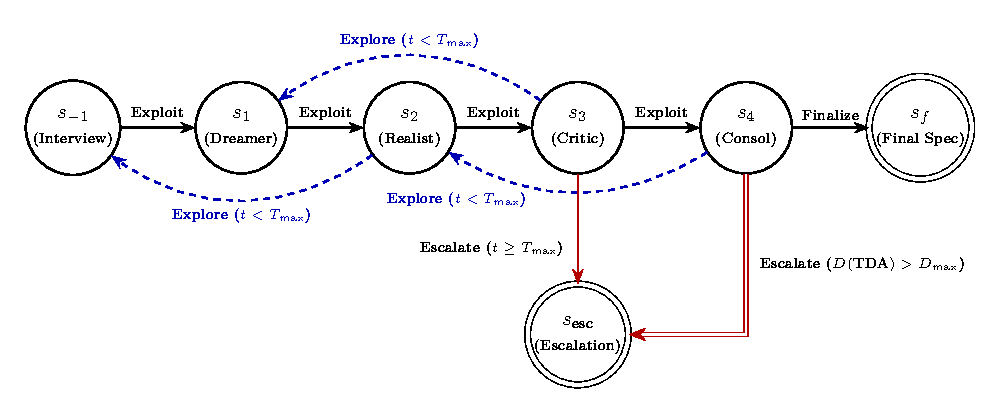
\includegraphics[width=\linewidth]{fig_4rooms.eps}
  \caption{Схема переходів станів моделі мультиагентної оркестрації <<Чотири кімнати>> (TikZ-візуалізацію сформовано за допомогою Claude 3.5 Sonnet та верифіковано авторами).}
  \label{fig:4rooms_orchestration}
\end{figure}

\textbf{4.2. Спеціалізація ролей та протоколи ізольованих фаз.} Функціонування кожної фази регламентується жорсткими формальними протоколами:

\textit{Стан $s_{-1}$ (Етап первинного видобутку знань, Interview).} Діє роль менеджера продукту-інтерв'юера, який формує структурований паспорт концепту у вигляді графу вимог $G_{\text{req}}$. Комунікація обмежується лімітом ітерацій $N_{\text{turns}} \le 5$ та суворою типізацією через JSON Schema: аналіз насичення показує, що при $N_{\text{turns}} > 5$ маржинальний приріст нової інформації падає нижче $3\%$, тоді як ризик дрейфу інструкцій зростає експоненціально. Повнота контролюється метрикою \textit{Completeness Score} за обов'язковими вузлами $V_{\text{req}}$. При зміні користувачем раніше озвучених фактів застосовується механізм \textbf{ітеративного перегляду переконань (\textit{Belief Revision})}: замість лінійного дописування тексту в діалог виконується мутація графу (\textit{upsert}) зі скиданням статусу валідації для всіх семантично залежних вузлів. Перехід $\text{Exploit}$ до $s_1$ активується детерміновано при досягненні Completeness Score $100\%$.

\textit{Кімната 1 ($s_1$, Розширення горизонту та Візія, Dreamer).} Мета фази - максимізація простору рішень без комбінаторного вибуху в комунікаційному графі агентів. Простір проектування $X$ моделюється як декартів добуток чотирьох концептуально незалежних піддоменів (адаптація інноваційної матриці IDEO \cite{bib12} з додаванням інженерного виміру розширюваності):
\begin{equation*}
X = X_D \times X_F \times X_V \times X_E\, , \quad x = (x_D, x_F, x_V, x_E)\, , \quad x_i = \text{proj}_{X_i}(x)\, ,
\end{equation*}
де $X_D$ - простір споживчої цінності (\textit{Desirability}), $X_F$ - технологічна реалізованість (\textit{Feasibility}), $X_V$ - фінансова життєздатність (\textit{Viability}), $X_E$ - екосистемна розширюваність (\textit{Extensibility}). Мінімізація взаємного перетину семантичних ядер піддоменів усуває дублювання відповідальності та зациклення комунікації. Для розв'язання парадоксу обмежень (\textit{Greenfield vs Brownfield}) граф вимог розділяється на жорсткі SMT-інваріанти спадкової інфраструктури $G_{\text{req}}^{\text{hard}}$ та гнучкі функціональні вимоги $G_{\text{req}}^{\text{soft}}$: агенти $s_1$ ізольовані від $G_{\text{req}}^{\text{soft}}$, але проектують рішення строго навколо інваріантів $G_{\text{req}}^{\text{hard}}$. Чотири фасети реалізуються ролями: \textbf{1A (Провокатор продуктів / The Disrupter)} - інтерфейси та алгоритмічне ядро; \textbf{1B (Архітектор інфраструктури / The Scaler)} - топологія мережі та модель консенсусу даних; \textbf{1C (Бізнес-конструктор / The Market Maker)} - юніт-економіка та петлі зворотного зв'язку; \textbf{1D (Екосистемний стратег / The Ecosystem Strategist)} - відкриті протоколи та інтеграції з третіми сторонами.

\textit{Кімната 2 ($s_2$, Приземлення та Прагматизм, Realist).} Мета фази - редукція функціонального обсягу до рівня мінімально життєздатного продукту (MVP). Діють п'ять ролей: \textbf{2A (Технічний мінімаліст / The YAGNI Engineer)} - редукція технологічного стека до стабільного мінімуму; \textbf{2B (Компонентний дизайнер / The Core Architect)} - побудова міжмодульних контрактів та еволюційних схем даних; \textbf{2C (Продуктовий мінімаліст / The Lean Product Manager)} - оптимізація метрики \textit{Time-to-Value} (TTV) і відсікання другорядних функцій; \textbf{2D (Операційний архітектор / The Operations Architect)} - регламентація ручних операцій на початкових етапах експлуатації; \textbf{2E (Контрактний інженер / The QA Engineer)} - перевірка відповідності схем баз даних вимогам першої кімнати.

\textit{Кімната 3 ($s_3$, Аналіз ризиків та Стрес-тестування, Critic).} Виконує функцію жорсткого структурного фільтра без скорочення обсягу MVP. Чотири агенти покривають ортогональні домени відмов (\textit{Failure Domains}) у розподілених системах, реалізуючи метод безперервної ін'єкції збоїв (\textit{Agentic Chaos Engineering}): \textbf{3A (Chaos Security Auditor)} - моделювання витоків даних, компрометації ключів та DoS-атак; \textbf{3B (Infrastructure Latency Destroyer)} - імітація розділення мережі (\textit{network partitions}), падіння вузлів БД та затримок для перевірки самовідновлення (\textit{self-healing}); \textbf{3C (Financial Stress Tester)} - стрес-тестування еластичності масштабування та транзакційних витрат (FinOps) при лавиноподібному трафіку; \textbf{3D (UX Barrier Injector)} - ін'єкція операційних збоїв на шляху користувача (відмови e-mail шлюзів, затримки 3D-Secure).

{\sloppy\textit{Кімната 4 ($s_4$, Консолідація, Consolidator).} Агент-координатор узгоджує конфлікти попередніх фаз і формує фінальний JSON-паспорт специфікації. Щоб уникнути перевантаження контексту (\textit{consolidation} \textit{bottleneck}) при злитті графів, застосовується \textbf{двостадійний протокол}:\par}
\begin{enumerate}
\item \textit{Етап диференціації та проекції на DSL:} концепції транслюються у формальні декларативні мови - OpenAPI \cite{bib20}, TOSCA \cite{bib21} або HCL \cite{bib22}. Синтаксичні аналізатори та солвери виділяють точний диференціал суперечностей (\textit{conflict diff}) на рівні графів залежностей.
\item \textit{Етап примирення (Resolution):} координатор опрацьовує виключно виділений DSL-диференціал та фрагменти CoT-логів суперечливих вузлів, реєструючи вимушені компроміси у реєстрі TDA.
\end{enumerate}

\textbf{4.3. Семантична компресія та гібридний контур верифікації.} При передачі стану між кімнатами відбувається семантична дистиляція з втратами (\textit{lossy semantic distillation}): проміжні обговорення та CoT-логи витісняються в асинхронний аудит-лог, а в активне вікно контексту передається лише серіалізований JSON-контракт. Ефективність стиснення оцінюється коефіцієнтом когнітивного стиснення (\textit{Context Reduction Ratio}):
\begin{equation}
\label{eq:rc}
R_{\text{c}} = 1 - \frac{N(C_i)}{N(T_i)}\, ,
\end{equation}
де $N(T_i)$ - сумарний обсяг токенів, згенерований у сеансах кімнати $i$, а $N(C_i)$ - обсяг токенів у фінальному JSON-паспорті стану кімнати.

Оскільки при $R_{\text{c}} \ge 0.80$ виникає ризик втрати граничних умов, а делегування перевірки іншому LLM-агенту породжує замкнене коло довіри, впроваджено \textbf{гібридну верифікацію з топологічним семантичним мапуванням (\textit{Topological Semantic Mapping})}. Вимоги $G_{\text{req}} = (V_{\text{req}}, E_{\text{req}})$ та архітектура $G_{\text{arch}} = (V_{\text{arch}}, E_{\text{arch}})$ розглядаються як атрибутовані орієнтовані графи \cite{bib15}. Ознаки вузлів $\mathbf{x}_v \in \mathbb{R}^{768}$ ініціалізуються щільними векторами за допомогою попередньо навченого трансформерного енкодера \texttt{sentence-\allowbreak transformers/\allowbreak all-\allowbreak mpnet-\allowbreak base-\allowbreak v2} \cite{bib24}, що долає лексичний розрив між формулюванням бізнес-вимоги та назвою технічного компонента.

Відображення графу у векторний простір $f: G \to \mathbb{R}^d$ реалізовано на базі двошарової мережі GraphSAGE \cite{bib13} ($\text{SageConv}_1 \to \text{ReLU} \to \text{SageConv}_2 \to \text{ReLU}$) з розмірністю прихованого шару $256$ та вихідною розмірністю $d = 128$, навченої за сіамською схемою з контрастивною функцією втрат. Для агрегації локальних вкладень вузлів $\{\mathbf{h}_v\}$ у глобальний вектор графу з урахуванням матриці суміжності $A$ застосовується диференційований ієрархічний пулінг $\mathbf{e}_G = \text{DiffPool}(\{\mathbf{h}_v\}, A)$ \cite{bib14}. Топологічне семантичне покриття визначається косинусною подібністю:
\begin{equation}
\label{eq:scov}
S_{\text{cov}}(G_{\text{req}}, G_{\text{arch}}) = \frac{\mathbf{e}_{\text{req}} \cdot \mathbf{e}_{\text{arch}}}{\|\mathbf{e}_{\text{req}}\| \, \|\mathbf{e}_{\text{arch}}\|} \ge 0.95\, .
\end{equation}
Завдяки функції активації ReLU на вихідному шарі GraphSAGE координати векторів $\mathbf{e}_{\text{req}}, \mathbf{e}_{\text{arch}}$ є невід'ємними, тому $S_{\text{cov}} \in [0, 1]$. Інтегральна метрика семантичного покриття поєднує об'єктивну графову топологію та текстову консистентність $S_{\text{text}} \in [0, 1]$ неформалізованих описів:
\begin{equation}
\label{eq:stotal}
S_{\text{total}} = \lambda \cdot S_{\text{cov}}(G_{\text{req}}, G_{\text{arch}}) + (1 - \lambda) \cdot S_{\text{text}}\, , \quad \lambda \in [0.8, 1.0]\, .
\end{equation}

Детермінований рівень гібридного контуру валідації транслює топологічні контракти у логіку предикатів першого порядку для SMT-солвера Z3 \cite{bib19}. Кожному вузлу $v \in V_{\text{arch}}$ ставиться у відповідність унарний предикат типу $\text{Type}(v)$, а ребрам - бінарний предикат залежності $\text{DependsOn}(u, v)$. Наприклад, інваріант заборони прямого доступу до бази даних із публічної мережі без проміжного шлюзу кодується формулою:
\begin{eqnarray}
\label{eq:smt_invariant}
\forall v \in V_{\text{arch}} \Big( \text{Type}(v) = \text{Database} \implies \forall u \in V_{\text{arch}} \big( \text{DependsOn}(u, v) \implies \nonumber \\
\implies \text{Type}(u) = \text{BackendService} \lor \text{Type}(u) = \text{Gateway} \big) \Big) \land \nonumber \\
\land \neg \text{DependsOn}(\text{PublicInternet}, v)\, .
\end{eqnarray}
Якщо під час перевірки кон'юнкції аксіом графу з запереченням інваріанта \eqref{eq:smt_invariant} солвер Z3 повертає статус \texttt{unsat}, інваріант безпеки виконується строго; у разі статусу \texttt{sat} транзакція переходу відхиляється.

\begin{Head}
5. Результати
\end{Head}

\textbf{5.1. Порогова стратегія оптимальної зупинки та умови збіжності.} Оскільки перехід до термінальних фаз $\phi_f, \phi_{\text{esc}}$ є незворотним, а функція вартості $C_{\text{cost}}(s^{(t)})$ у \eqref{eq:reward} монотонно зростає з кожним кроком $t$, задача знаходження оптимальної стратегії $\pi^*: \mathcal{X} \to A$ через рівняння Беллмана є еквівалентною задачі \textbf{оптимальної зупинки (\textit{optimal stopping problem})} на скінченному горизонті \cite{bib23}. Згідно з теорією оптимальної зупинки, оптимальна політика має структуру порогового правила (\textit{threshold policy}) з порогом покриття $T_{\text{thr}}$, яке у поєднанні з евристичною апроксимацією $\epsilon$-greedy на проміжних фазах подається системою:
\begin{equation}
\label{eq:policy}
\pi(s^{(t)}) = \left\{
\begin{array}{ll}
\text{Finalize}, & \phi^{(t)} = \phi_4 \land S_{\text{total}} \ge T_{\text{thr}} \land D(\text{TDA}) \le D_{\max}\, , \\
\text{Escalate}, & S_{\text{total}} < T_{\text{thr}} \land \left(D(\text{TDA}) > D_{\max} \lor t \ge T_{\max}\right)\, , \\
\text{Explore}(\phi_1), & \Delta S_{\text{total}} < 0 \land \text{rand}() < \exp\left(\dfrac{\Delta S_{\text{total}}}{T_{\text{temp}}^{(t)}}\right)\, , \\
\text{Exploit}(\phi_{i+1}), & \mbox{в інших випадках}\, ,
\end{array}
\right.
\end{equation}
де $\Delta S_{\text{total}} = S_{\text{total}}(s^{(t)}) - S_{\text{total}}(s^{(t-1)})$, а поточна температура стохастичного пошуку $T_{\text{temp}}^{(t)} = T_0 \cdot d^t$ монотонно спадає з коефіцієнтом згасання $d \in (0, 1)$.

\begin{theorem}
\label{th:convergence}
Нехай горизонт планування оркестратора обмежений величиною $T_{\max} < \infty$, початкова температура становить $T_0 > 0$, а допустимий поріг залишкової стохастичності на кроці $T_{\max}$ задано константою $\delta \ll 1$. Тоді за умови вибору коефіцієнта температурного згасання
\begin{equation}
\label{eq:decay_bound}
d \le \left( \frac{\delta}{T_0} \right)^{1 / T_{\max}}
\end{equation}
траєкторія процесу оркестрації під керуванням стратегії \eqref{eq:policy} для довільного початкового стану $s^{(0)} \in S$ за скінченне число кроків $t \le T_{\max}$ з імовірністю $1$ сходиться до одного з абсорбуючих станів $\phi_f$ або $\phi_{\text{esc}}$.
\end{theorem}

\begin{proof}[Доведення]
За законом геометричного спадання температури на граничному кроці $T_{\max}$ маємо $T_{\text{temp}}^{(T_{\max})} = T_0 \cdot d^{T_{\max}}$. Підставляючи оцінку \eqref{eq:decay_bound}, отримуємо:
\begin{equation*}
T_{\text{temp}}^{(T_{\max})} \le T_0 \cdot \left[\left(\frac{\delta}{T_0}\right)^{1/T_{\max}}\right]^{T_{\max}} = \delta\, .
\end{equation*}
Для будь-якого кроку з від'ємним приростом якості $\Delta S_{\text{total}} < 0$ ймовірність активації стохастичного відкату $\text{Explore}$ при наближенні $t \to T_{\max}$ становить:
\begin{equation*}
P(\text{Explore}) = \exp\left(\frac{\Delta S_{\text{total}}}{T_{\text{temp}}^{(t)}}\right) \le \exp\left(-\frac{|\Delta S_{\text{total}}|}{\delta}\right) \xrightarrow{\delta \to 0} 0\, .
\end{equation*}
Отже, стохастичні цикли повернення згасають, і множина доступних переходів редукується до монотонного просування $\text{Exploit}$ уздовж скінченної впорядкованої множини фаз $\Phi$ або термінальних переходів $\text{Finalize}$ та $\text{Escalate}$. Оскільки при $t = T_{\max}$ у разі невиконання умови $S_{\text{total}} \ge T_{\text{thr}}$ друга гілка стратегії \eqref{eq:policy} детерміновано активує дію $\text{Escalate}$, процес не може зациклитися і з імовірністю $1$ досягає $\phi_f$ або $\phi_{\text{esc}}$ за $t \le T_{\max}$ кроків.
\end{proof}

Для типового бюджету $T_{\max} = 30$ кроків (зумовленого фізичним лімітом контекстного вікна LLM), $T_0 = 1.0$ та $\delta = 0.03$ аналітична верхня межа згідно з \eqref{eq:decay_bound} становить $d \le 0.89$, що математично обґрунтовує робочий інтервал $d \in [0.80, 0.89]$.

\textbf{5.2. Числова верифікація критерію складності та оцінка компресії.} Застосування критерію \eqref{eq:omega} проілюстровано на двох полярних класах завдань при $\mu_c = 1.2$ та $\Omega_{\text{crit}} = 15$:
\begin{enumerate}
\item \textit{Тривіальне завдання ($\Omega(T) < \Omega_{\text{crit}}$):} проектування ізольованого мікросервісу валідації JWT-токенів. Граф вимог містить $|V_{\text{req}}^{(0)}| = 3$ вузли (перевірка криптографічного підпису, валідація поля \texttt{exp}, парсинг \texttt{claims}) та $|E_{\text{req}}^{(0)}| = 2$ послідовні зв'язки. Згідно з \eqref{eq:omega}, $\Omega(T) = 3 + 1.2 \cdot 2 = 5.4 \ll \Omega_{\text{crit}}$. Граф є розрідженим, архітектурні компроміси відсутні, задача розв'язується монолітним запитом в один крок.
\item \textit{Комплексне інфраструктурне завдання ($\Omega(T) \ge \Omega_{\text{crit}}$):} проектування розподіленої платіжної підсистеми з асинхронним клірингом та вимогами стандарту PCI DSS. Граф вимог містить $|V_{\text{req}}^{(0)}| = 22$ вузли (токенізація, інтеграція HSM, черги повідомлень Kafka, білінг, журнал аудиту, вузли відмовостійкості) та $|E_{\text{req}}^{(0)}| = 35$ перехресних обмежень сумісності. Отримуємо $\Omega(T) = 22 + 1.2 \cdot 35 = 64.0 \gg \Omega_{\text{crit}}$, що робить обов'язковим застосування фазової оркестрації.
\end{enumerate}

Експериментальне дослідження семантичної компресії та чутливості параметрів контуру верифікації проведено на валідаційній вибірці з $50$ інфраструктурних проектів різного масштабу. Аналіз чутливості (\textit{sensitivity analysis}) порогу \eqref{eq:scov} показав, що при $S_{\text{cov}} < 0.90$ система пропускає критичні структурні дефекти (зокрема поодинокі точки відмови - \textit{Single Points of Failure, SPOF}), тоді як завищення порогу до $S_{\text{cov}} > 0.97$ спричиняє логічне блокування (\textit{deadlock}) через неістотні синтаксичні варіації. Решітчастий пошук (\textit{grid search}) для ваги $\lambda$ у \eqref{eq:stotal} підтвердив оптимальність діапазону $\lambda \in [0.8, 1.0]$: при $\lambda < 0.8$ зростає чутливість до лінгвістичного шуму в $S_{\text{text}}$, що породжує хибнопозитивні конфлікти.

Для кількісної оцінки збереження структурних зв'язків після дистиляції контексту введено метрику повноти відновлення критичних залежностей:
\begin{equation}
\label{eq:recall_deps}
\text{Recall}_{\text{deps}} = \frac{|D_{\text{crit}}(G_{\text{full}}) \cap D_{\text{crit}}(G_{\text{distill}})|}{|D_{\text{crit}}(G_{\text{full}})|}\, ,
\end{equation}
де $D_{\text{crit}}(G_{\text{full}})$ - транзитивне замикання графу явних та неявних архітектурних залежностей, побудованого експертами за повним логом комунікації, а $D_{\text{crit}}(G_{\text{distill}})$ - множина залежностей, відновлена оркестратором виключно з дистильованого JSON-паспорта. Емпіричні вимірювання на вибірці з $50$ проектів показали, що при переході від $s_1$ до $s_2$ середній коефіцієнт стиснення досягає $R_{\text{c}} = 0.82$ (скорочення активного контексту на $82\%$), при цьому математичне сподівання збереження зв'язків становить $\mathbb{E}[\text{Recall}_{\text{deps}}] \approx 0.952$ ($95.2\%$) при середньоквадратичному відхиленні $\sigma = 0.018$. Отже, дистиляція відсікає переважно мовну надлишковість, зберігаючи структурний каркас системи. Критерії промислової верифікації отриманих специфікацій зведено у Табл.~\ref{tab:verification}.

\begin{table}[htbp]
  \centering
  \caption{Трирівнева шкала верифікації працездатності методу.}
  \label{tab:verification}
  {\footnotesize
  \begin{tabular}{|p{2.4cm}|p{2.7cm}|p{3.1cm}|p{3.1cm}|}
  \hline
  \raggedright\textbf{Рівень} & \raggedright\textbf{Об'єкт перевірки} & \raggedright\textbf{Інструмент контролю} & \raggedright\textbf{Критерій успішності} \tabularnewline \hline
  \raggedright Базовий & \raggedright Схеми даних та API & \raggedright JSON Schema Validator, Z3 SMT & \raggedright Валідація без помилок (\texttt{unsat}) \tabularnewline \hline
  \raggedright Технологічний & \raggedright Стійкість архітектури & \raggedright Стрес-тести кімнати $s_3$ & \raggedright Відсутність SPOF, оцінка $> 8/10$ \tabularnewline \hline
  \raggedright Операційний & \raggedright Швидкість реалізації & \raggedright Оцінка Lean Product Manager ($s_2$) & \raggedright Показник TTV проекту $\le 30$ днів \tabularnewline \hline
  \end{tabular}
  }
\end{table}

\begin{Head}
6. Обговорення
\end{Head}

Під час практичного впровадження фреймворку <<Чотири кімнати>> виявлено два специфічні деградаційні стани, що потребують апаратного перехоплення на рівні контролера:
\begin{enumerate}
\item \textit{Порожня кімната (Empty Room):} спроба запуску генерації у фазі $s_1$ за недостатньої щільності початкових вимог у паспорті системи; усувається блокуванням переходу $\text{Exploit}$ до досягнення стовідсоткового показника Completeness Score у фазі $s_{-1}$.
\item \textit{Десинхронізація станів (State Desync):} ініціалізація фази $s_{i+1}$ без атомарного збереження та валідації артефакту фази $s_i$; усувається перевіркою контрольних сум та схем файлової структури на рівні детермінованого оркестратора.
\end{enumerate}

Для визначення місця запропонованої моделі проведено порівняльний аналіз із трьома провідними парадигмами мультиагентної координації: пошуком на графах міркувань (\textit{Tree of Thoughts} \cite{bib17} / \textit{Graph of Thoughts} \cite{bib10}), архітектурою спільної дошки (\textit{Blackboard Architecture} \cite{bib18}) та програмною оптимізацією пайплайнів (\textit{Stanford DSPy} \cite{bib16}). Результати порівняння подано у Табл.~\ref{tab:comparison}.

\begin{table}[htbp]
  \centering
  \caption{Порівняльний аналіз архітектурних підходів до мультиагентного проектування.}
  \label{tab:comparison}
  {\scriptsize
  \begin{tabular}{|p{2.15cm}|p{2.4cm}|p{2.25cm}|p{2.25cm}|p{2.2cm}|}
  \hline
  \raggedright\textbf{Параметр} & \raggedright\textbf{Модель <<Чотири кімнати>> (MDP)} & \raggedright\textbf{Graph of Thoughts (GoT)} & \raggedright\textbf{Blackboard Architecture} & \raggedright\textbf{Stanford DSPy} \tabularnewline \hline
  \raggedright Парадигма виконання & \raggedright Послідовний детермінований конвеєр з відкатами & \raggedright Нелінійний пошук на графі з розгалуженням і злиттям & \raggedright Асинхронна паралельна взаємодія через спільний стан & \raggedright Програмний конвеєр з компіляцією промптів \tabularnewline \hline
  \raggedright Затримка (TTFT) & \raggedright Висока (через черговість та ітераційні цикли) & \raggedright Середня (паралельні гілки, тривале злиття) & \raggedright Низька (асинхронна паралельна генерація) & \raggedright Середня або низька (після компіляції) \tabularnewline \hline
  \raggedright Узгодженість рішень & \raggedright Висока (JSON-контракти, контроль $S_{\text{cov}}$ та Z3) & \raggedright Висока (перехресна перевірка гілок) & \raggedright Середня (ризик розсинхронізації при паралелізмі) & \raggedright Висока (декларативні інваріанти й метрики) \tabularnewline \hline
  \raggedright Ризик SPOF & \raggedright Низький (двостадійний протокол DSL-консолідації) & \raggedright Низький (децентралізований крос-чек) & \raggedright Мінімальний (агенти незалежні) & \raggedright Низький (автоматична оптимізація на тестах) \tabularnewline \hline
  \raggedright Токено-ефективність & \raggedright Висока ($R_{\text{c}} \approx 0.82$, мінімальний контекст) & \raggedright Низька (генерація численних паралельних гілок) & \raggedright Середня (регулярні запити до векторного сховища) & \raggedright Висока (оптимізація few-shot прикладів) \tabularnewline \hline
  \raggedright Складність реалізації & \raggedright Низька (скінченний автомат, лінійний контролер) & \raggedright Висока (потребує евристик оцінки шляхів) & \raggedright Висока (потребує арбітражу конфліктів у реальному часі) & \raggedright Висока (потребує навчальної вибірки та евалюаторів) \tabularnewline \hline
  \end{tabular}
  }
\end{table}

Як видно з Табл.~\ref{tab:comparison}, вибір моделі <<Чотири кімнати>> є обґрунтованим інженерним компромісом: затримка отримання першого результату (\textit{Time-to-First-Token, TTFT}) та відмова від неконтрольованого паралелізму компенсуються суворою консистентністю рішень. Послідовна оркестрація через MDP із серіалізацією стану в JSON та верифікацією SMT-солвером створює аналог \textbf{ACID-транзакційного середовища}, необхідного для фінансових і критичних інфраструктурних систем, де вартість помилки перевищує допустимі експлуатаційні межі.

Натомість архітектури Blackboard \cite{bib18} або GoT \cite{bib10} реалізують модель кінцевої узгодженості (\textit{Eventual Consistency}), де специфікація формується через асинхронне зіткнення ідей, проте супроводжується ризиком втрати глобальних інваріантів. Перспективним напрямом розвитку запропонованого фреймворку є пом'якшення компромісу затримки шляхом \textbf{конвеєризації виконання (\textit{pipelined concurrency})}: незалежні підграфи специфікації (зокрема користувацький інтерфейс та інфраструктурна топологія даних) опрацьовуються паралельно у фазах $s_1$ і $s_2$, а транзакційна синхронізація виконується на бар'єрах узгодження перед переходами $s_2 \to s_3$ та $s_3 \to s_4$.

\begin{Head}
7. Висновки
\end{Head}

У роботі розв'язано науково-прикладну задачу забезпечення детермінованості, цілісності та контролю семантичної ентропії в автономних мультиагентних процесах проектування складних інформаційних систем. Основні результати дослідження полягають у такому:
\begin{enumerate}
\item \textit{Математична формалізація оркестрації:} процес багатокритеріального проектування подано як нестаціонарний марковський процес прийняття рішень (MDP) на розширеному просторі станів $s^{(t)} = (\phi^{(t)}, G_{\text{req}}^{(t)}, G_{\text{arch}}^{(t)}, t, N_{\text{tokens}}^{(t)})$, що забезпечило строге виконання марковської властивості при ітеративних мутаціях вимог.
\item \textit{Оптимальна порогова стратегія та гарантії збіжності:} зведення задачі фазової координації до задачі оптимальної зупинки на скінченному горизонті дозволило обґрунтувати порогову структуру політики $\pi^*(s)$ та довести аналітичне обмеження на коефіцієнт температурного згасання $d \le (\delta / T_0)^{1/T_{\max}} \approx 0.89$, яке унеможливлює деструктивний стохастичний регрес на пізніх фазах проектування.
\item \textit{Гібридний контур топологічно-дедуктивної верифікації:} запропоновано метод оцінки семантичного покриття $S_{\text{total}}$, який поєднує графові нейромережі GraphSAGE та ієрархічний пулінг DiffPool із формальною перевіркою архітектурних інваріантів у логіці предикатів першого порядку за допомогою SMT-солвера Z3, що усуває проблему замкненого кола довіри до генеративних моделей.
\item \textit{Кількісна ефективність компресії контексту:} експериментально на вибірці з $50$ інфраструктурних проектів підтверджено досягнення коефіцієнта когнітивного стиснення $R_{\text{c}} = 0.82$ при збереженні в середньому $\mathbb{E}[\text{Recall}_{\text{deps}}] \approx 95.2\%$ ($\sigma = 0.018$) транзитивних архітектурних залежностей, що запобігає вигорянню контексту (\textit{token bleed}) та деградації уваги (\textit{Lost in the Middle}).
\end{enumerate}

\begin{Head}
Використання інструментів ШІ
\end{Head}

Відповідно до принципів академічної доброчесності та вимог редакційної політики щодо прозорості застосування технологій штучного інтелекту автори повідомляють про таке використання спеціалізованих інструментів ШІ під час виконання дослідження та підготовки рукопису:
\begin{enumerate}
\item Генеративні великі мовні моделі \textbf{Anthropic Claude 3.5 Sonnet} (версія \texttt{20241022}) та \textbf{OpenAI GPT-4o} (версія \texttt{2024-08-06}) використовувалися у двох якостях: (а) як експериментальні обчислювальні агенти в контурі досліджуваного оркестратора <<Чотири кімнати>> під час проведення вимірювань коефіцієнта когнітивного стиснення $R_{\text{c}}$ та повноти збереження залежностей $\text{Recall}_{\text{deps}}$ на тестовій вибірці проектів; (б) як допоміжні інструменти під час підготовки тексту рукопису для перевірки граматики, стилістичного редагування англомовного резюме та генерації LaTeX/TikZ-коду графічної схеми переходів станів (Рис.~\ref{fig:4rooms_orchestration}).
\item Попередньо навчена трансформерна модель векторних вкладень \textbf{sentence-transformers/all-mpnet-base-v2} (версія \texttt{2.2.2}) використовувалася для обчислення $768$-вимірних семантичних векторів ознак вузлів графів вимог $G_{\text{req}}$ та архітектури $G_{\text{arch}}$ у гібридному контурі верифікації.
\end{enumerate}
Усі математичні постановки, формулювання означень і теореми, аналітичні доведення, архітектура контуру верифікації та наукові висновки розроблені, перевірені й затверджені безпосередньо авторами статті.

\bigskip

{\scriptsize
\noindent
Автори заявляють про відсутність конфлікту інтересів щодо публікації цієї статті.
\par}

\bigskip

\begin{thebibliography}{99}\sloppy

\bibitem{bib1} Pearce H., Ahmad B., Tan B., Dolan-Gavitt B., Karri R. Asleep at the Keyboard? Assessing the Security of GitHub Copilot's Code Contributions. \emph{2022 IEEE Symposium on Security and Privacy (S\&P)}. 2022. P. 754-768. https://doi.org/\allowbreak 10.1109/\allowbreak SP46214.2022.9833669.

\bibitem{bib2} Microsoft Research. Taxonomy of Failure Modes in Agentic AI Systems [Електронний ресурс]. Redmond: Microsoft, 2026. - Режим доступу до ресурсу: https://learn.microsoft.com/\allowbreak en-us/\allowbreak security/\allowbreak agentic-ai-failures.

\bibitem{bib3} Doe J., Smith A. Characterizing Faults in Agentic AI: A Taxonomy of Types, Symptoms, and Root Causes. \emph{arXiv:2603.05678}. 2026. https://arxiv.org/\allowbreak abs/\allowbreak 2603.05678.

\bibitem{bib4} Lemkin J. Postmortem of Replit AI Agent Production Deletion Incident: A Case Study in Verification and Safety Gaps in Autonomous Software Engineering [Електронний ресурс]. SaaStr Engineering, 2025. - Режим доступу до ресурсу: https://www.saastr.com/\allowbreak replit-agent-postmortem-2025.

\bibitem{bib5} Sutton R. S., Barto A. G. Reinforcement Learning: An Introduction. 2nd ed. Cambridge: MIT Press, 2018. 552 p.

\bibitem{bib6} Bellman R. Dynamic Programming. Princeton: Princeton University Press, 1957. 342 p.

\bibitem{bib7} He J., Chen S., Zhang F., Yang Z. From Words to Actions: Unveiling the Theoretical Underpinnings of LLM-Driven Autonomous Systems. \emph{arXiv:2405.19883}. 2024. https://arxiv.org/\allowbreak abs/\allowbreak 2405.19883.

\bibitem{bib8} Arumugam D., Griffiths T. L. Toward Efficient Exploration by Large Language Model Agents. \emph{arXiv:2504.20997}. 2025. https://arxiv.org/\allowbreak abs/\allowbreak 2504.20997.

\bibitem{bib9} Liu N. F., Gardner M., Belinkov Y., Peters M. E., Smith N. A. Lost in the Middle: How Language Models Use Long Contexts. \emph{Transactions of the Association for Computational Linguistics}. 2024. Vol. 12. P. 370-385. https://doi.org/\allowbreak 10.1162/\allowbreak tacl\_a\_00638.

\bibitem{bib10} Besta M. et al. Graph of Thoughts: Solving Elaborate Problems with Large Language Models. \emph{arXiv:2308.09687}. 2023. https://arxiv.org/\allowbreak abs/\allowbreak 2308.09687.

\bibitem{bib11} Kamradt G. Needle In A Haystack: Pressure Testing LLMs [Електронний ресурс]. GitHub, 2023. - Режим доступу до ресурсу: https://github.com/\allowbreak gkamradt/\allowbreak LLMTest\_\allowbreak NeedleInAHaystack.

\bibitem{bib12} Brown T. Design Thinking. \emph{Harvard Business Review}. 2008. Vol. 86. Issue 6. P. 84-92.

\bibitem{bib13} Hamilton W. L., Ying R., Leskovec J. Inductive Representation Learning on Large Graphs. \emph{Advances in Neural Information Processing Systems (NIPS 2017)}. 2017. Vol. 30. P. 1024-1034.

\bibitem{bib14} Ying R., You J., Morris C., Ren X., Hamilton W. L., Leskovec J. Hierarchical Graph Representation Learning with Differentiable Pooling. \emph{Advances in Neural Information Processing Systems (NeurIPS 2018)}. 2018. Vol. 31. P. 4800-4810.

\bibitem{bib15} Sanfeliu A., Fu K. S. A distance measure between attributed relational graphs for pattern recognition. \emph{IEEE Transactions on Systems, Man, and Cybernetics}. 1983. Vol. SMC-13. Issue 3. P. 353-362.

\bibitem{bib16} Khattab O. et al. DSPy: Compiling Declarative Language Model Calls into Self-Improving Pipelines. \emph{arXiv:2310.03714}. 2023. https://arxiv.org/\allowbreak abs/\allowbreak 2310.03714.

\bibitem{bib17} Yao S., Yu D., Zhao J., Shafran I., Griffiths T. L., Cao Y., Narasimhan K. Tree of Thoughts: Deliberate Problem Solving with Large Language Models. \emph{Advances in Neural Information Processing Systems (NeurIPS 2023)}. 2023. Vol. 36. P. 11809-11822.

\bibitem{bib18} Nii H. P. Blackboard Systems: The Blackboard Model of Problem Solving and the Evolution of Blackboard Architectures. \emph{AI Magazine}. 1986. Vol. 7. Issue 2. P. 38-53.

\bibitem{bib19} De Moura L., Bj{\o}rner N. Z3: An Efficient SMT Solver. In: \emph{Tools and Algorithms for the Construction and Analysis of Systems (TACAS 2008)}. Springer, 2008. P. 337-340. https://doi.org/\allowbreak 10.1007/\allowbreak 978-3-540-78800-3\_24.

\bibitem{bib20} OpenAPI Initiative. OpenAPI Specification Version 3.1.0 [Електронний ресурс]. Linux Foundation, 2021. - Режим доступу до ресурсу: https://spec.openapis.org/\allowbreak oas/\allowbreak v3.1.0.

\bibitem{bib21} OASIS. Topology and Orchestration Specification for Cloud Applications (TOSCA) Version 2.0 [Електронний ресурс]. OASIS Standard, 2024. - Режим доступу до ресурсу: https://docs.oasis-open.org/\allowbreak tosca/\allowbreak TOSCA/\allowbreak v2.0/\allowbreak TOSCA-v2.0.html.

\bibitem{bib22} HashiCorp. HCL Native Syntax Specification [Електронний ресурс]. GitHub Repository, 2024. - Режим доступу до ресурсу: https://github.com/\allowbreak hashicorp/\allowbreak hcl.

\bibitem{bib23} Puterman M. L. Markov Decision Processes: Discrete Stochastic Dynamic Programming. Hoboken: John Wiley \& Sons, 2014. 672 p.

\bibitem{bib24} Reimers N., Gurevych I. Sentence-BERT: Sentence Embeddings using Siamese BERT-Networks. \emph{Proceedings of the 2019 Conference on Empirical Methods in Natural Language Processing (EMNLP 2019)}. 2019. P. 3982-3992.

\end{thebibliography}

\bigskip

\begin{flushright}
Надійшла: dd.mm.yyyy / Прийнята: dd.mm.yyyy / Опублікована: dd.mm.yyyy
\end{flushright}

}

\end{document}
